\section{Angriffsmethoden}
\subsection{Ablauf}
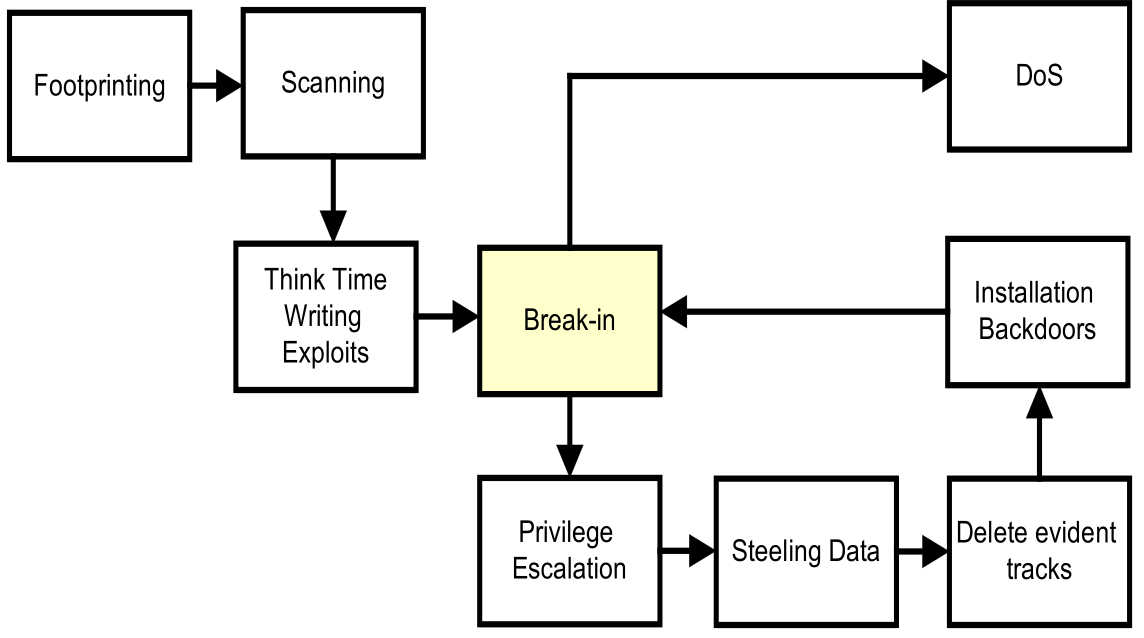
\includegraphics[width=\linewidth]{angriffsmethoden.png}

\subsection{Direkte Attacken}
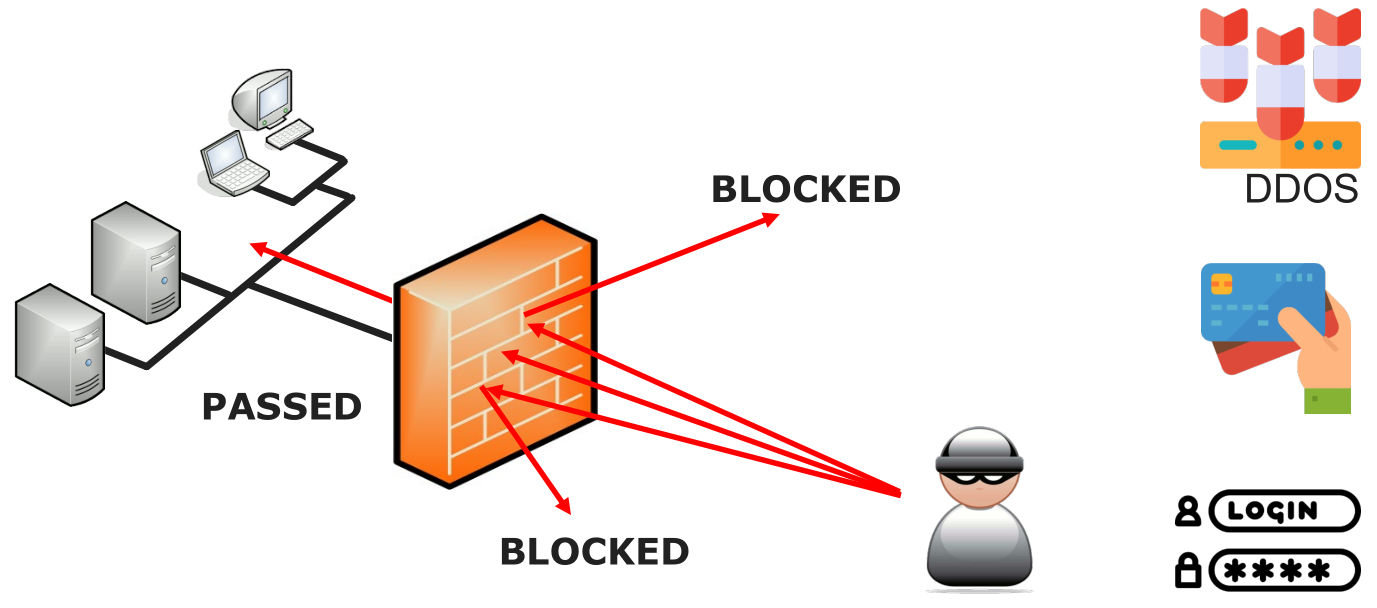
\includegraphics[width=\linewidth]{direct-attack.png}
Beispiele:
\begin{itemize}
  \item DoS
  \item Brute Forcing a Password
  \item Password Spraying
\end{itemize}

\subsection{Indirekte Attacken}
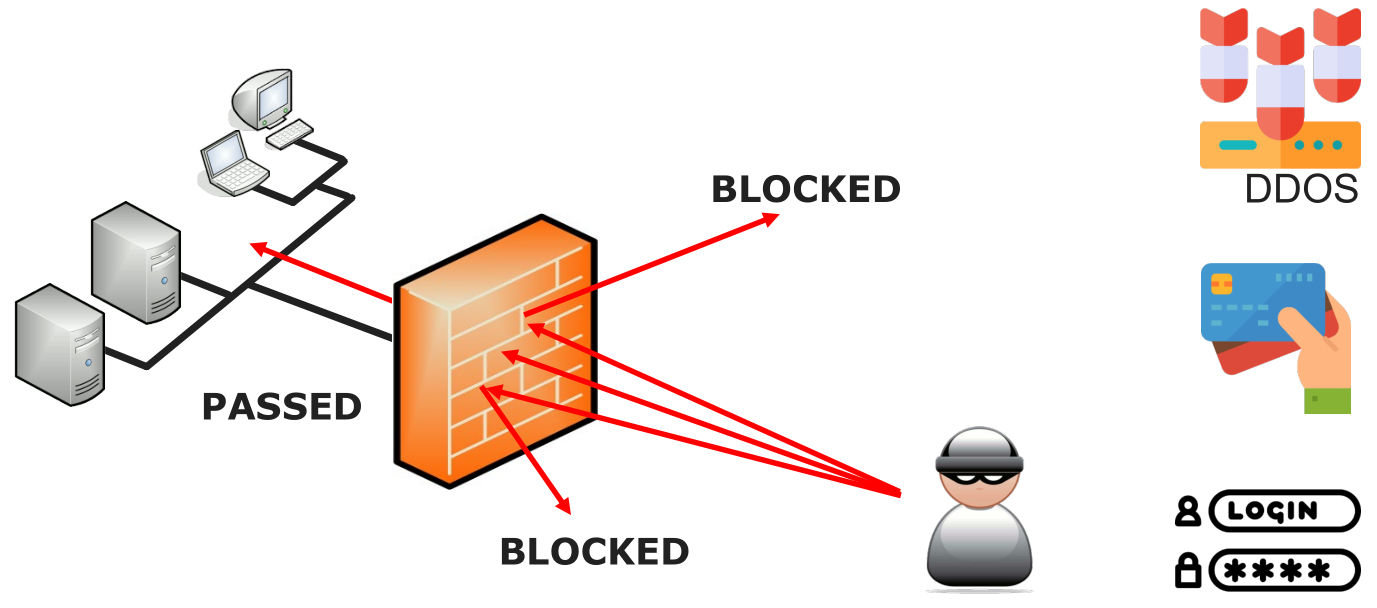
\includegraphics[width=\linewidth]{direct-attack.png}
Beispiele:
\begin{itemize}
  \item Virus
  \item Malware 
  \item Ransomware
\end{itemize}

\subsection{Man in the Middle}
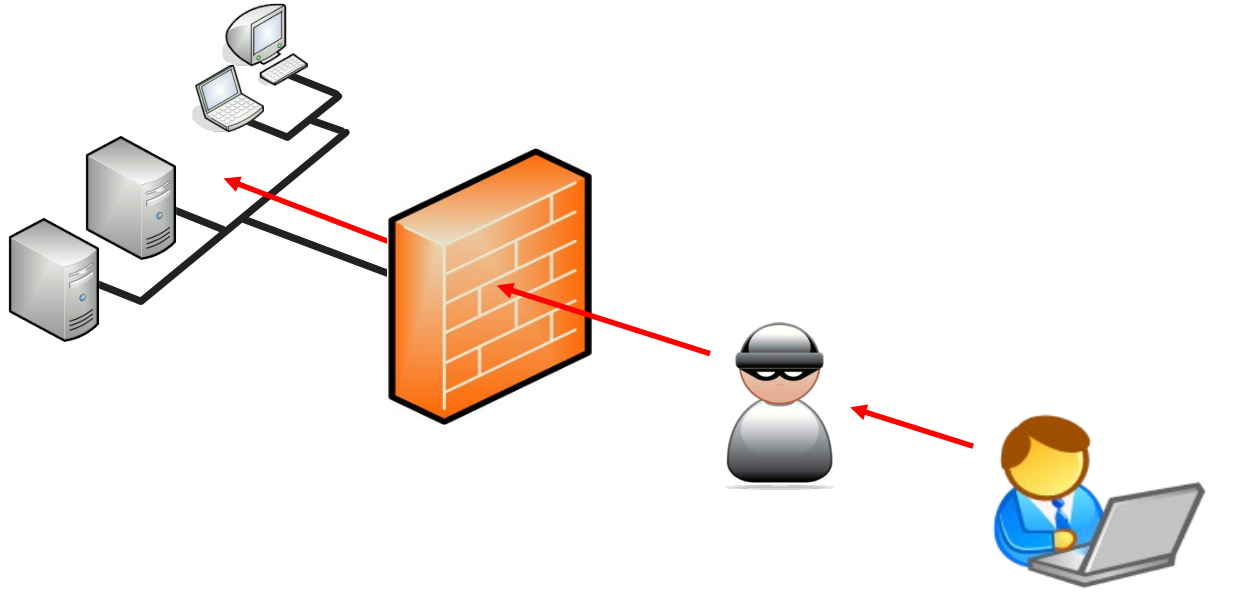
\includegraphics[width=\linewidth]{mitm-attack.png}\\
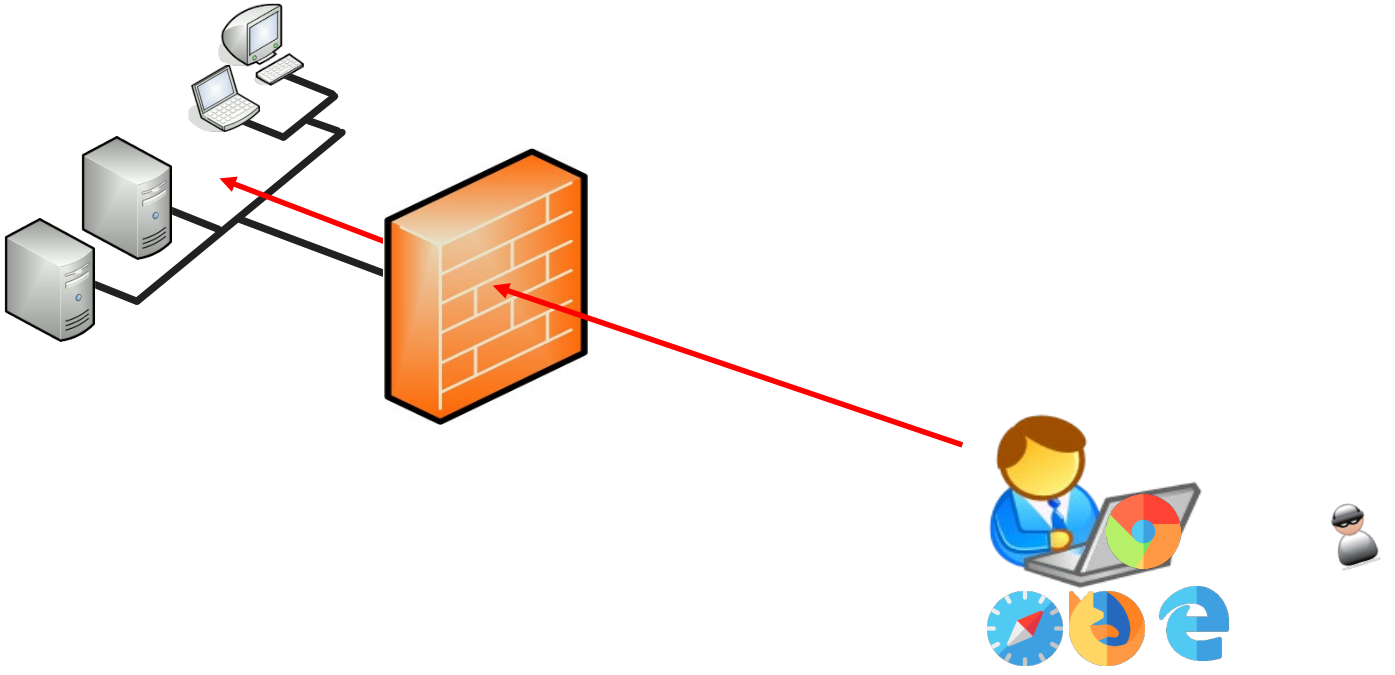
\includegraphics[width=\linewidth]{mitb-attack.png}\\
Mehr unter %TODO: Add chapter

\subsection{Privilege Elevation}
Die Ausweitung von Berechtigungen ist ein gängiger Bedrohungsvektor für Angreifer, der es ihnen ermöglicht, in die IT-Infrastruktur von Unternehmen einzudringen und Berechtigungen zu erlangen, um sensible Daten zu stehlen, den Betrieb zu stören und Hintertüren für zukünftige Angriffe zu schaffen. 
Erhöhte Berechtigungen öffnen Angreifern Tür und Tor, um Sicherheitseinstellungen, Konfigurationen und Daten zu manipulieren. Häufig verschaffen sie sich zunächst Zugang zu Konten mit niedrigeren Berechtigungen und nutzen diese dann, um höhere Berechtigungen zu erlangen und vollen Zugriff auf die IT-Umgebung des Unternehmens zu erhalten.\\

\subsubsection{Gängie Methoden}
\paragraph{Linux:}
\begin{itemize}
  \item Enumeration
  \item Kernel-Exploits
  \item SUDO Right Exploitation
\end{itemize}
\paragraph{Windows:}
\begin{itemize}
  \item Access Token Manipulation
  \item Bypass User Account Control
\end{itemize}

\subsection{Social Engineering}
Social Engineering ist eine Bedrohung der Cybersicherheit, die das schwächste Glied in unserer Sicherheitskette - unsere Mitarbeiter - ausnutzt, um Zugang zu Unternehmensnetzwerken zu erhalten. 
Angreifer nutzen immer raffiniertere Tricks und emotionale Manipulation, um Mitarbeiter, sogar Führungskräfte, dazu zu bringen, sensible Informationen preiszugeben.

\subsubsection{Gängie Methoden}
\textbf{Informationen sind nicht aus der Vorlesung!}
\paragraph{Phising}
Bei einem Phishing-Angriff verwendet ein Angreifer eine Nachricht, die er per E-Mail, über soziale Medien, Instant-Messaging-Clients oder SMS verschickt, um sensible Informationen von einem Opfer zu erhalten oder es dazu zu bringen, auf einen Link zu einer bösartigen Website zu klicken.

\paragraph{Watering hole}
Bei einem Watering-Hole-Angriff wird bösartiger Code von einer legitimen Website aus gestartet oder heruntergeladen, die von den Zielpersonen des Angriffs häufig besucht wird. Angreifer könnten beispielsweise eine Nachrichtenseite aus der Finanzbranche kompromittieren, da sie wissen, dass Personen, die im Finanzwesen arbeiten und somit ein attraktives Ziel darstellen, diese Seite wahrscheinlich besuchen. Auf der kompromittierten Website wird in der Regel ein Backdoor-Trojaner installiert, der es dem Angreifer ermöglicht, das Gerät des Opfers zu kompromittieren und fernzusteuern.

\paragraph{Whaling attack / Spear-Phising}
Whaling, auch bekannt als Spear-Phishing, ist eine Art von Phishing-Angriff, der auf bestimmte Personen mit privilegiertem Zugang zu Systemen oder mit Zugang zu äußerst wertvollen sensiblen Informationen abzielt. Ein Whaling-Angriff kann beispielsweise gegen leitende Angestellte, wohlhabende Personen oder Netzwerkadministratoren durchgeführt werden.

\paragraph{Pretexting}
Bei einem Pretexting-Angriff geben sich die Angreifer mit einer gefälschten Identität aus, um ihre Opfer zur Herausgabe privater Informationen zu verleiten. Die Angreifer können sich beispielsweise als externer IT-Dienstleister ausgeben und die Kontodaten und Passwörter der Benutzer anfordern, um ihnen bei einem Problem zu helfen.

\paragraph{Baiting and quid pro quo attacks}
Bei einem Köderangriff bieten die Angreifer etwas an, von dem die Opfer glauben, dass es nützlich ist. Dabei kann es sich um ein vermeintliches Software-Update handeln, bei dem es sich in Wirklichkeit um eine bösartige Datei handelt, oder um einen infizierten USB-Token mit einem Etikett, das darauf hinweist, dass er wertvolle Informationen enthält, und andere Methoden.


\subsection{MITRE ATT\&CK Framework}
Mehr unter %TODO: Add chapter

\subsection{APT}
Advanced Persistent Threat ist ein häufig im Bereich der Cyber-Bedrohung (Cyber-Attacke) verwendeter Begriff für einen komplexen, zielgerichteten und effektiven Angriff auf kritische IT-Infrastrukturen und vertrauliche Daten von Behörden, Groß- und Mittelstandsunternehmen aller Branchen, welche aufgrund ihres Technologievorsprungs potenzielle Opfer darstellen oder als Sprungbrett auf solche Opfer dienen können.

\subsubsection{Problematik}
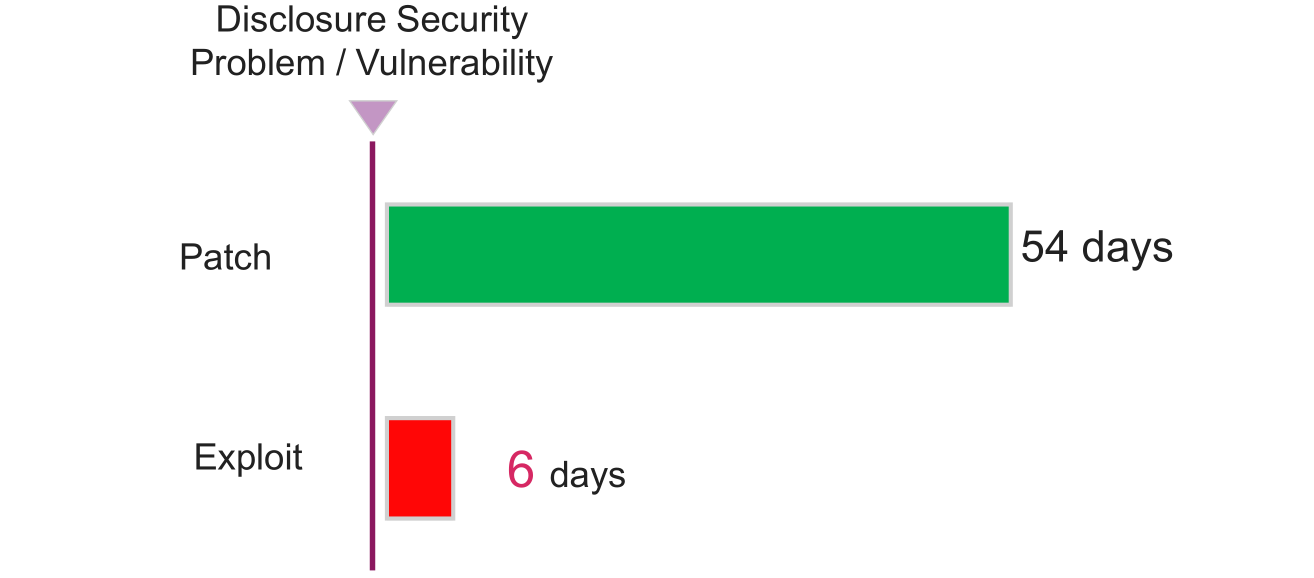
\includegraphics[width=\linewidth]{apt-disclosure.png}\\
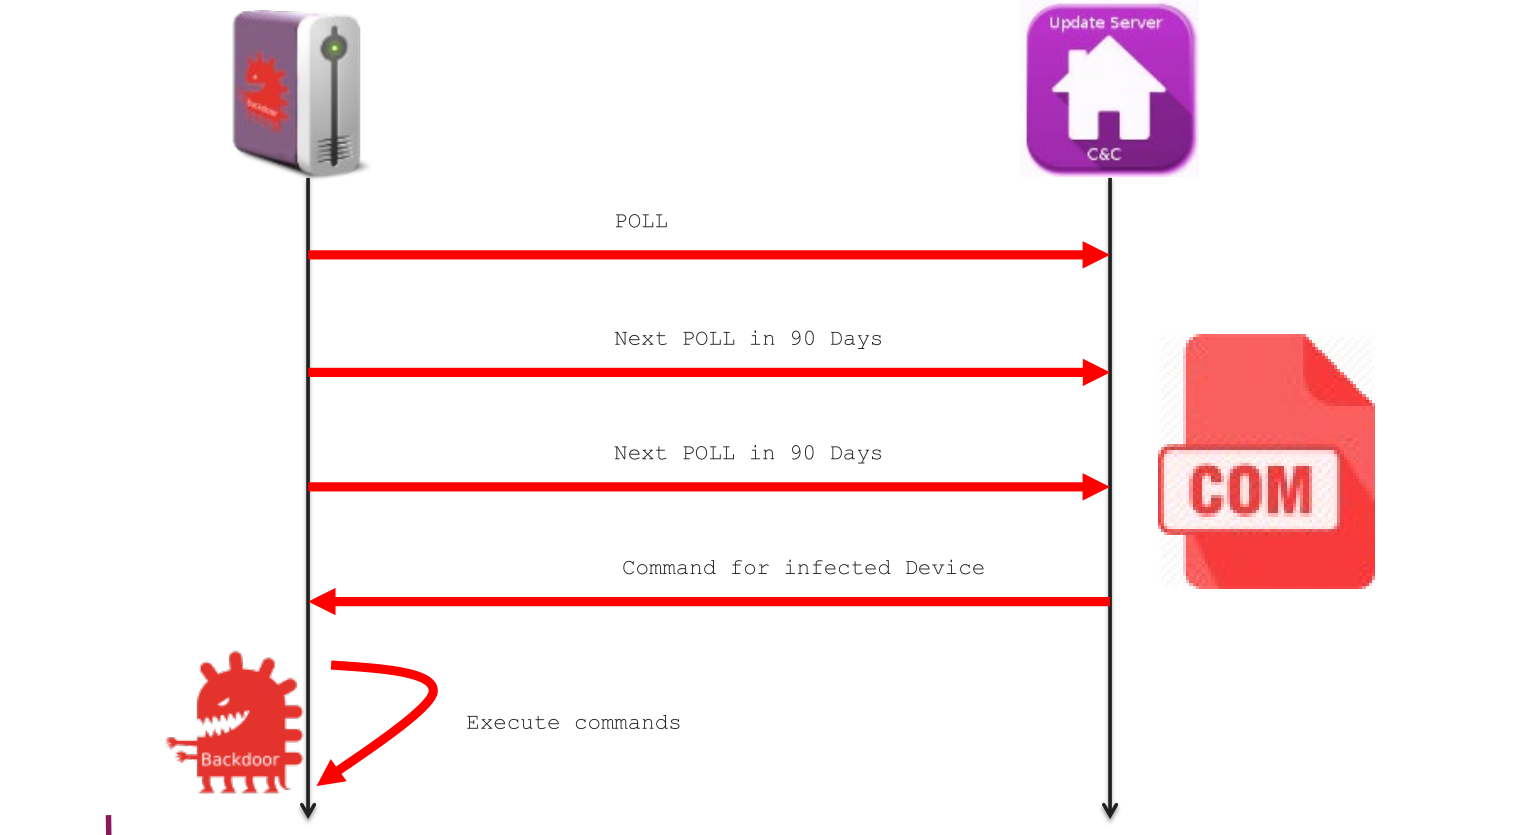
\includegraphics[width=\linewidth]{apt-time-frame.png}

\subsubsection{Fünf Stages}
\paragraph{1: Gain Access}
Wie ein Einbrecher, der eine Tür mit einem Brecheisen aufbricht, verschaffen sich Cyberkriminelle in der Regel über ein Netzwerk, eine infizierte Datei, eine Junk-E-Mail oder eine App-Schwachstelle Zugang, um Malware in ein Zielnetzwerk einzuschleusen.

\paragraph{2: Establish a Foothold}
Cyberkriminelle implantieren Malware, die die Schaffung eines Netzwerks von Hintertüren und Tunneln ermöglicht, um sich unbemerkt in Systemen zu bewegen. Die Malware verwendet oft Techniken wie das Umschreiben von Code, um den Hackern zu helfen, ihre Spuren zu verwischen.

\paragraph{3: Deepen Access}
Wenn sie erst einmal drin sind, nutzen Hacker Techniken wie das Knacken von Passwörtern, um sich Zugang zu Administratorrechten zu verschaffen, damit sie mehr Kontrolle über das System haben und noch mehr Zugriff erhalten.

\paragraph{4: Laterally Movement}
Tiefer im System, mit Administratorrechten, können sich Hacker nach Belieben bewegen. 
Sie können auch versuchen, auf andere Server und andere sichere Teile des Netzes zuzugreifen.

\paragraph{5: Look, Learn, and Remain}
Aus dem Inneren des Systems heraus erhalten die Hacker ein umfassendes Verständnis seiner Funktionsweise und seiner Schwachstellen, was es ihnen ermöglicht, die gewünschten Informationen nach Belieben zu sammeln.

\subsubsection{Erkennung}
\paragraph{Logging}
\begin{itemize}
  \item DNS Resolution
  \item HTTP/S Logging
  \item E-Mail Logging
\end{itemize}

\paragraph{Lookup Services}
\begin{itemize}
  \item Block\&Black
  \item Mandiant
  \item ZEUS TRACKER
  \item Malware Hash
  \item OpenIOC
  \item IP Reputation
\end{itemize}

\subsubsection{Methoden}
Siehe Kapitel %TODO: Add chapter Red-Teaming